\section{options.h File Reference}
\label{options_8h}\index{options.h@{options.h}}


This graph shows which files directly or indirectly include this file:\nopagebreak
\begin{figure}[H]
\begin{center}
\leavevmode
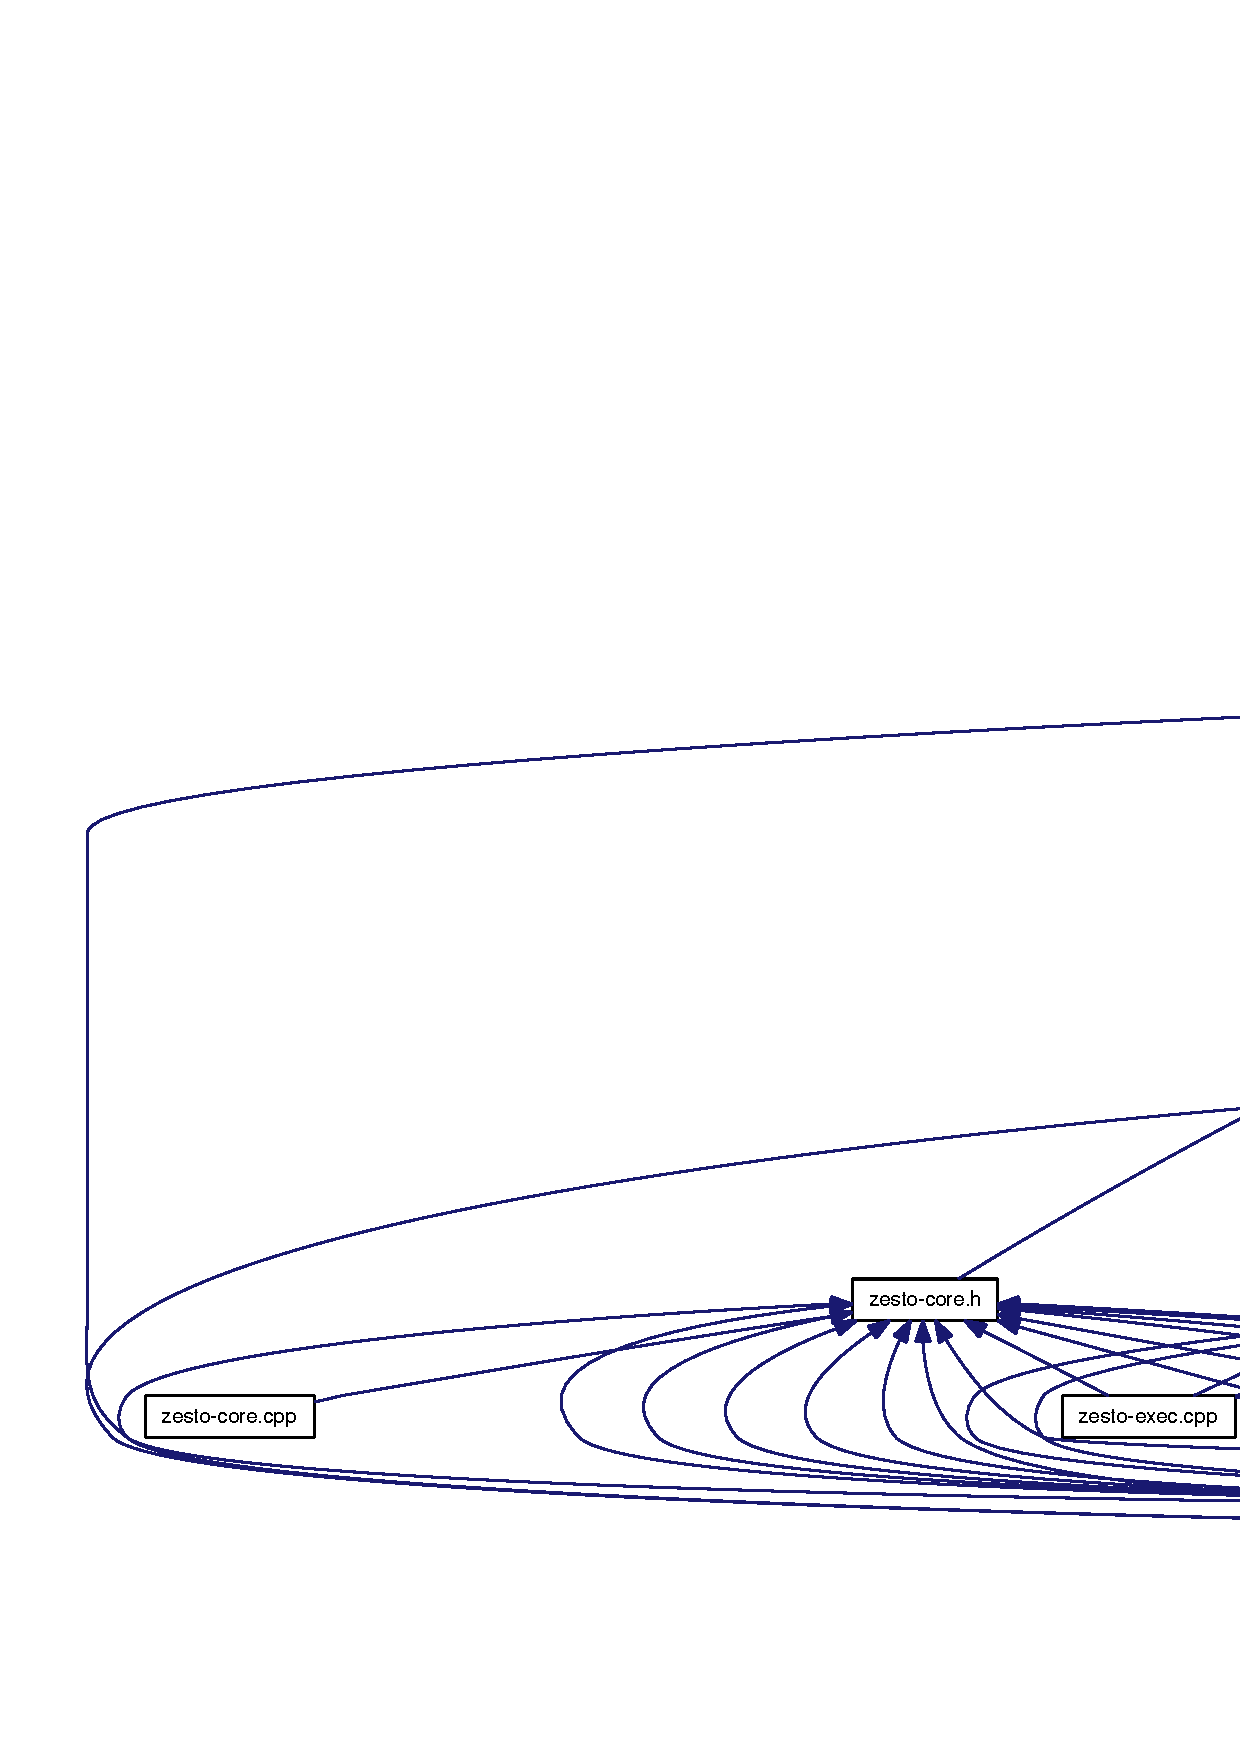
\includegraphics[width=420pt]{options_8h__dep__incl}
\end{center}
\end{figure}
\subsection*{Classes}
\begin{CompactItemize}
\item 
struct {\bf opt\_\-opt\_\-t}
\item 
union {\bf opt\_\-opt\_\-t::opt\_\-opt\_\-t::opt\_\-variant\_\-t}
\item 
struct {\bf opt\_\-opt\_\-t::opt\_\-opt\_\-t::opt\_\-variant\_\-t::opt\_\-opt\_\-t::opt\_\-variant\_\-t::opt\_\-for\_\-int\_\-t}
\item 
struct {\bf opt\_\-opt\_\-t::opt\_\-opt\_\-t::opt\_\-variant\_\-t::opt\_\-opt\_\-t::opt\_\-variant\_\-t::opt\_\-for\_\-uint\_\-t}
\item 
struct {\bf opt\_\-opt\_\-t::opt\_\-opt\_\-t::opt\_\-variant\_\-t::opt\_\-opt\_\-t::opt\_\-variant\_\-t::opt\_\-for\_\-float\_\-t}
\item 
struct {\bf opt\_\-opt\_\-t::opt\_\-opt\_\-t::opt\_\-variant\_\-t::opt\_\-opt\_\-t::opt\_\-variant\_\-t::opt\_\-for\_\-double\_\-t}
\item 
struct {\bf opt\_\-opt\_\-t::opt\_\-opt\_\-t::opt\_\-variant\_\-t::opt\_\-opt\_\-t::opt\_\-variant\_\-t::opt\_\-for\_\-enum\_\-t}
\item 
struct {\bf opt\_\-opt\_\-t::opt\_\-opt\_\-t::opt\_\-variant\_\-t::opt\_\-opt\_\-t::opt\_\-variant\_\-t::opt\_\-for\_\-string\_\-t}
\item 
struct {\bf opt\_\-opt\_\-t::opt\_\-opt\_\-t::opt\_\-variant\_\-t::opt\_\-opt\_\-t::opt\_\-variant\_\-t::opt\_\-for\_\-long\_\-long\_\-t}
\item 
struct {\bf opt\_\-note\_\-t}
\item 
struct {\bf opt\_\-odb\_\-t}
\end{CompactItemize}
\subsection*{Typedefs}
\begin{CompactItemize}
\item 
typedef int($\ast$ {\bf orphan\_\-fn\_\-t} )(int i, int argc, char $\ast$$\ast$argv)
\end{CompactItemize}
\subsection*{Enumerations}
\begin{CompactItemize}
\item 
enum {\bf opt\_\-class\_\-t} \{ \par
{\bf oc\_\-int} =  0, 
{\bf oc\_\-uint}, 
{\bf oc\_\-float}, 
{\bf oc\_\-double}, 
\par
{\bf oc\_\-enum}, 
{\bf oc\_\-flag}, 
{\bf oc\_\-string}, 
{\bf oc\_\-long\_\-long}, 
\par
{\bf oc\_\-NUM}
 \}
\end{CompactItemize}
\subsection*{Functions}
\begin{CompactItemize}
\item 
struct {\bf opt\_\-odb\_\-t} $\ast$ {\bf opt\_\-new} ({\bf orphan\_\-fn\_\-t} orphan\_\-fn)
\item 
void {\bf opt\_\-delete} (struct {\bf opt\_\-odb\_\-t} $\ast$odb)
\item 
void {\bf opt\_\-reg\_\-long\_\-long} (struct {\bf opt\_\-odb\_\-t} $\ast$odb, char $\ast$name, char $\ast$desc, long long $\ast$var, long long def\_\-val, int print, char $\ast$format)
\item 
void {\bf opt\_\-reg\_\-int} (struct {\bf opt\_\-odb\_\-t} $\ast$odb, char $\ast$name, char $\ast$desc, int $\ast$var, int def\_\-val, int print, char $\ast$format)
\item 
void {\bf opt\_\-reg\_\-int\_\-list} (struct {\bf opt\_\-odb\_\-t} $\ast$odb, char $\ast$name, char $\ast$desc, int $\ast$vars, int nvars, int $\ast$nelt, int $\ast$def\_\-val, int print, char $\ast$format, int accrue)
\item 
void {\bf opt\_\-reg\_\-uint} (struct {\bf opt\_\-odb\_\-t} $\ast$odb, char $\ast$name, char $\ast$desc, unsigned int $\ast$var, unsigned int def\_\-val, int print, char $\ast$format)
\item 
void {\bf opt\_\-reg\_\-uint\_\-list} (struct {\bf opt\_\-odb\_\-t} $\ast$odb, char $\ast$name, char $\ast$desc, unsigned int $\ast$vars, int nvars, int $\ast$nelt, unsigned int $\ast$def\_\-val, int print, char $\ast$format, int accrue)
\item 
void {\bf opt\_\-reg\_\-float} (struct {\bf opt\_\-odb\_\-t} $\ast$odb, char $\ast$name, char $\ast$desc, float $\ast$var, float def\_\-val, int print, char $\ast$format)
\item 
void {\bf opt\_\-reg\_\-float\_\-list} (struct {\bf opt\_\-odb\_\-t} $\ast$odb, char $\ast$name, char $\ast$desc, float $\ast$vars, int nvars, int $\ast$nelt, float $\ast$def\_\-val, int print, char $\ast$format, int accrue)
\item 
void {\bf opt\_\-reg\_\-double} (struct {\bf opt\_\-odb\_\-t} $\ast$odb, char $\ast$name, char $\ast$desc, double $\ast$var, double def\_\-val, int print, char $\ast$format)
\item 
void {\bf opt\_\-reg\_\-double\_\-list} (struct {\bf opt\_\-odb\_\-t} $\ast$odb, char $\ast$name, char $\ast$desc, double $\ast$vars, int nvars, int $\ast$nelt, double $\ast$def\_\-val, int print, char $\ast$format, int accrue)
\item 
void {\bf opt\_\-reg\_\-enum} (struct {\bf opt\_\-odb\_\-t} $\ast$odb, char $\ast$name, char $\ast$desc, int $\ast$var, char $\ast$def\_\-val, char $\ast$$\ast$emap, int $\ast$eval, int emap\_\-sz, int print, char $\ast$format)
\item 
void {\bf opt\_\-reg\_\-enum\_\-list} (struct {\bf opt\_\-odb\_\-t} $\ast$odb, char $\ast$name, char $\ast$desc, int $\ast$vars, int nvars, int $\ast$nelt, char $\ast$def\_\-val, char $\ast$$\ast$emap, int $\ast$eval, int emap\_\-sz, int print, char $\ast$format, int accrue)
\item 
void {\bf opt\_\-reg\_\-flag} (struct {\bf opt\_\-odb\_\-t} $\ast$odb, char $\ast$name, char $\ast$desc, bool $\ast$var, bool def\_\-val, int print, char $\ast$format)
\item 
void {\bf opt\_\-reg\_\-flag\_\-list} (struct {\bf opt\_\-odb\_\-t} $\ast$odb, char $\ast$name, char $\ast$desc, bool $\ast$vars, int nvars, int $\ast$nelt, bool $\ast$def\_\-val, int print, char $\ast$format, int accrue)
\item 
void {\bf opt\_\-reg\_\-string} (struct {\bf opt\_\-odb\_\-t} $\ast$odb, char $\ast$name, char $\ast$desc, char $\ast$$\ast$var, char $\ast$def\_\-val, int print, char $\ast$format)
\item 
void {\bf opt\_\-reg\_\-string\_\-list} (struct {\bf opt\_\-odb\_\-t} $\ast$odb, char $\ast$name, char $\ast$desc, char $\ast$$\ast$vars, int nvars, int $\ast$nelt, char $\ast$$\ast$def\_\-val, int print, char $\ast$format, int accrue)
\item 
void {\bf opt\_\-process\_\-options} (struct {\bf opt\_\-odb\_\-t} $\ast$odb, int argc, char $\ast$$\ast$argv)
\item 
void {\bf opt\_\-print\_\-option} (struct {\bf opt\_\-opt\_\-t} $\ast$opt, FILE $\ast$fd)
\item 
void {\bf opt\_\-print\_\-options} (struct {\bf opt\_\-odb\_\-t} $\ast$odb, FILE $\ast$fd, int terse, int notes)
\item 
void {\bf opt\_\-print\_\-help} (struct {\bf opt\_\-odb\_\-t} $\ast$odb, FILE $\ast$fd)
\item 
struct {\bf opt\_\-opt\_\-t} $\ast$ {\bf opt\_\-find\_\-option} (struct {\bf opt\_\-odb\_\-t} $\ast$odb, char $\ast$opt\_\-name)
\item 
void {\bf opt\_\-reg\_\-header} (struct {\bf opt\_\-odb\_\-t} $\ast$odb, char $\ast$header)
\item 
void {\bf opt\_\-reg\_\-note} (struct {\bf opt\_\-odb\_\-t} $\ast$odb, char $\ast$note)
\end{CompactItemize}
\subsection*{Variables}
\begin{CompactItemize}
\item 
bool {\bf opt\_\-ignore\_\-notes}
\end{CompactItemize}


\subsection{Typedef Documentation}
\index{options.h@{options.h}!orphan\_\-fn\_\-t@{orphan\_\-fn\_\-t}}
\index{orphan\_\-fn\_\-t@{orphan\_\-fn\_\-t}!options.h@{options.h}}
\subsubsection[{orphan\_\-fn\_\-t}]{\setlength{\rightskip}{0pt plus 5cm}typedef int($\ast$ {\bf orphan\_\-fn\_\-t})(int i,int argc,char $\ast$$\ast$argv)}\label{options_8h_14d29551e8d9d50370f93d6f1729fee4}




Definition at line 133 of file options.h.

\subsection{Enumeration Type Documentation}
\index{options.h@{options.h}!opt\_\-class\_\-t@{opt\_\-class\_\-t}}
\index{opt\_\-class\_\-t@{opt\_\-class\_\-t}!options.h@{options.h}}
\subsubsection[{opt\_\-class\_\-t}]{\setlength{\rightskip}{0pt plus 5cm}enum {\bf opt\_\-class\_\-t}}\label{options_8h_df032dd28ab2078e196d20be488993ab}


\begin{Desc}
\item[Enumerator: ]\par
\begin{description}
\index{oc\_\-int@{oc\_\-int}!options.h@{options.h}}\index{options.h@{options.h}!oc\_\-int@{oc\_\-int}}\item[{\em 
oc\_\-int\label{options_8h_df032dd28ab2078e196d20be488993ab9c249ce922a06a82cee15f739d11546b}
}]\index{oc\_\-uint@{oc\_\-uint}!options.h@{options.h}}\index{options.h@{options.h}!oc\_\-uint@{oc\_\-uint}}\item[{\em 
oc\_\-uint\label{options_8h_df032dd28ab2078e196d20be488993ab92effe4aab20d9aec5c1d00942d7d8e7}
}]\index{oc\_\-float@{oc\_\-float}!options.h@{options.h}}\index{options.h@{options.h}!oc\_\-float@{oc\_\-float}}\item[{\em 
oc\_\-float\label{options_8h_df032dd28ab2078e196d20be488993ab7657a926e8645bb4bcaf1b3d8d8d0d32}
}]\index{oc\_\-double@{oc\_\-double}!options.h@{options.h}}\index{options.h@{options.h}!oc\_\-double@{oc\_\-double}}\item[{\em 
oc\_\-double\label{options_8h_df032dd28ab2078e196d20be488993ab7e426d8cff2e2edae9ad2298be666b5a}
}]\index{oc\_\-enum@{oc\_\-enum}!options.h@{options.h}}\index{options.h@{options.h}!oc\_\-enum@{oc\_\-enum}}\item[{\em 
oc\_\-enum\label{options_8h_df032dd28ab2078e196d20be488993aba54214493d08e5392dd17173c22ca02c}
}]\index{oc\_\-flag@{oc\_\-flag}!options.h@{options.h}}\index{options.h@{options.h}!oc\_\-flag@{oc\_\-flag}}\item[{\em 
oc\_\-flag\label{options_8h_df032dd28ab2078e196d20be488993ab216b559c1b72f57e53e3d4f741d5c621}
}]\index{oc\_\-string@{oc\_\-string}!options.h@{options.h}}\index{options.h@{options.h}!oc\_\-string@{oc\_\-string}}\item[{\em 
oc\_\-string\label{options_8h_df032dd28ab2078e196d20be488993ab9eeb2921478a88d3d612d89193cbb8bc}
}]\index{oc\_\-long\_\-long@{oc\_\-long\_\-long}!options.h@{options.h}}\index{options.h@{options.h}!oc\_\-long\_\-long@{oc\_\-long\_\-long}}\item[{\em 
oc\_\-long\_\-long\label{options_8h_df032dd28ab2078e196d20be488993abb498ba433d26a6b83a8f5eea93c0bf5a}
}]\index{oc\_\-NUM@{oc\_\-NUM}!options.h@{options.h}}\index{options.h@{options.h}!oc\_\-NUM@{oc\_\-NUM}}\item[{\em 
oc\_\-NUM\label{options_8h_df032dd28ab2078e196d20be488993ab9e2e699f6d98b16f21ca7ab72a6ae15d}
}]\end{description}
\end{Desc}



Definition at line 73 of file options.h.

\subsection{Function Documentation}
\index{options.h@{options.h}!opt\_\-delete@{opt\_\-delete}}
\index{opt\_\-delete@{opt\_\-delete}!options.h@{options.h}}
\subsubsection[{opt\_\-delete}]{\setlength{\rightskip}{0pt plus 5cm}void opt\_\-delete (struct {\bf opt\_\-odb\_\-t} $\ast$ {\em odb})}\label{options_8h_446211e014d8f5668b0c4ab1eeb463d2}


\index{options.h@{options.h}!opt\_\-find\_\-option@{opt\_\-find\_\-option}}
\index{opt\_\-find\_\-option@{opt\_\-find\_\-option}!options.h@{options.h}}
\subsubsection[{opt\_\-find\_\-option}]{\setlength{\rightskip}{0pt plus 5cm}struct {\bf opt\_\-opt\_\-t}$\ast$ opt\_\-find\_\-option (struct {\bf opt\_\-odb\_\-t} $\ast$ {\em odb}, \/  char $\ast$ {\em opt\_\-name})\hspace{0.3cm}{\tt  [read]}}\label{options_8h_78c3c1709a2ce86dce11dcd2b5b2ae86}


\index{options.h@{options.h}!opt\_\-new@{opt\_\-new}}
\index{opt\_\-new@{opt\_\-new}!options.h@{options.h}}
\subsubsection[{opt\_\-new}]{\setlength{\rightskip}{0pt plus 5cm}struct {\bf opt\_\-odb\_\-t}$\ast$ opt\_\-new ({\bf orphan\_\-fn\_\-t} {\em orphan\_\-fn})\hspace{0.3cm}{\tt  [read]}}\label{options_8h_d900f5594c7d1ad23aa395b5dc9b5931}




Referenced by main().

Here is the caller graph for this function:\nopagebreak
\begin{figure}[H]
\begin{center}
\leavevmode
\includegraphics[width=85pt]{options_8h_d900f5594c7d1ad23aa395b5dc9b5931_icgraph}
\end{center}
\end{figure}
\index{options.h@{options.h}!opt\_\-print\_\-help@{opt\_\-print\_\-help}}
\index{opt\_\-print\_\-help@{opt\_\-print\_\-help}!options.h@{options.h}}
\subsubsection[{opt\_\-print\_\-help}]{\setlength{\rightskip}{0pt plus 5cm}void opt\_\-print\_\-help (struct {\bf opt\_\-odb\_\-t} $\ast$ {\em odb}, \/  FILE $\ast$ {\em fd})}\label{options_8h_e73e967de719b2d753404d9db58cc143}




Referenced by usage().

Here is the caller graph for this function:\nopagebreak
\begin{figure}[H]
\begin{center}
\leavevmode
\includegraphics[width=137pt]{options_8h_e73e967de719b2d753404d9db58cc143_icgraph}
\end{center}
\end{figure}
\index{options.h@{options.h}!opt\_\-print\_\-option@{opt\_\-print\_\-option}}
\index{opt\_\-print\_\-option@{opt\_\-print\_\-option}!options.h@{options.h}}
\subsubsection[{opt\_\-print\_\-option}]{\setlength{\rightskip}{0pt plus 5cm}void opt\_\-print\_\-option (struct {\bf opt\_\-opt\_\-t} $\ast$ {\em opt}, \/  FILE $\ast$ {\em fd})}\label{options_8h_49f9e748dd4b97535490958b7510de20}


\index{options.h@{options.h}!opt\_\-print\_\-options@{opt\_\-print\_\-options}}
\index{opt\_\-print\_\-options@{opt\_\-print\_\-options}!options.h@{options.h}}
\subsubsection[{opt\_\-print\_\-options}]{\setlength{\rightskip}{0pt plus 5cm}void opt\_\-print\_\-options (struct {\bf opt\_\-odb\_\-t} $\ast$ {\em odb}, \/  FILE $\ast$ {\em fd}, \/  int {\em terse}, \/  int {\em notes})}\label{options_8h_86b86016ad1396461ed934c0ab462a35}




Referenced by main().

Here is the caller graph for this function:\nopagebreak
\begin{figure}[H]
\begin{center}
\leavevmode
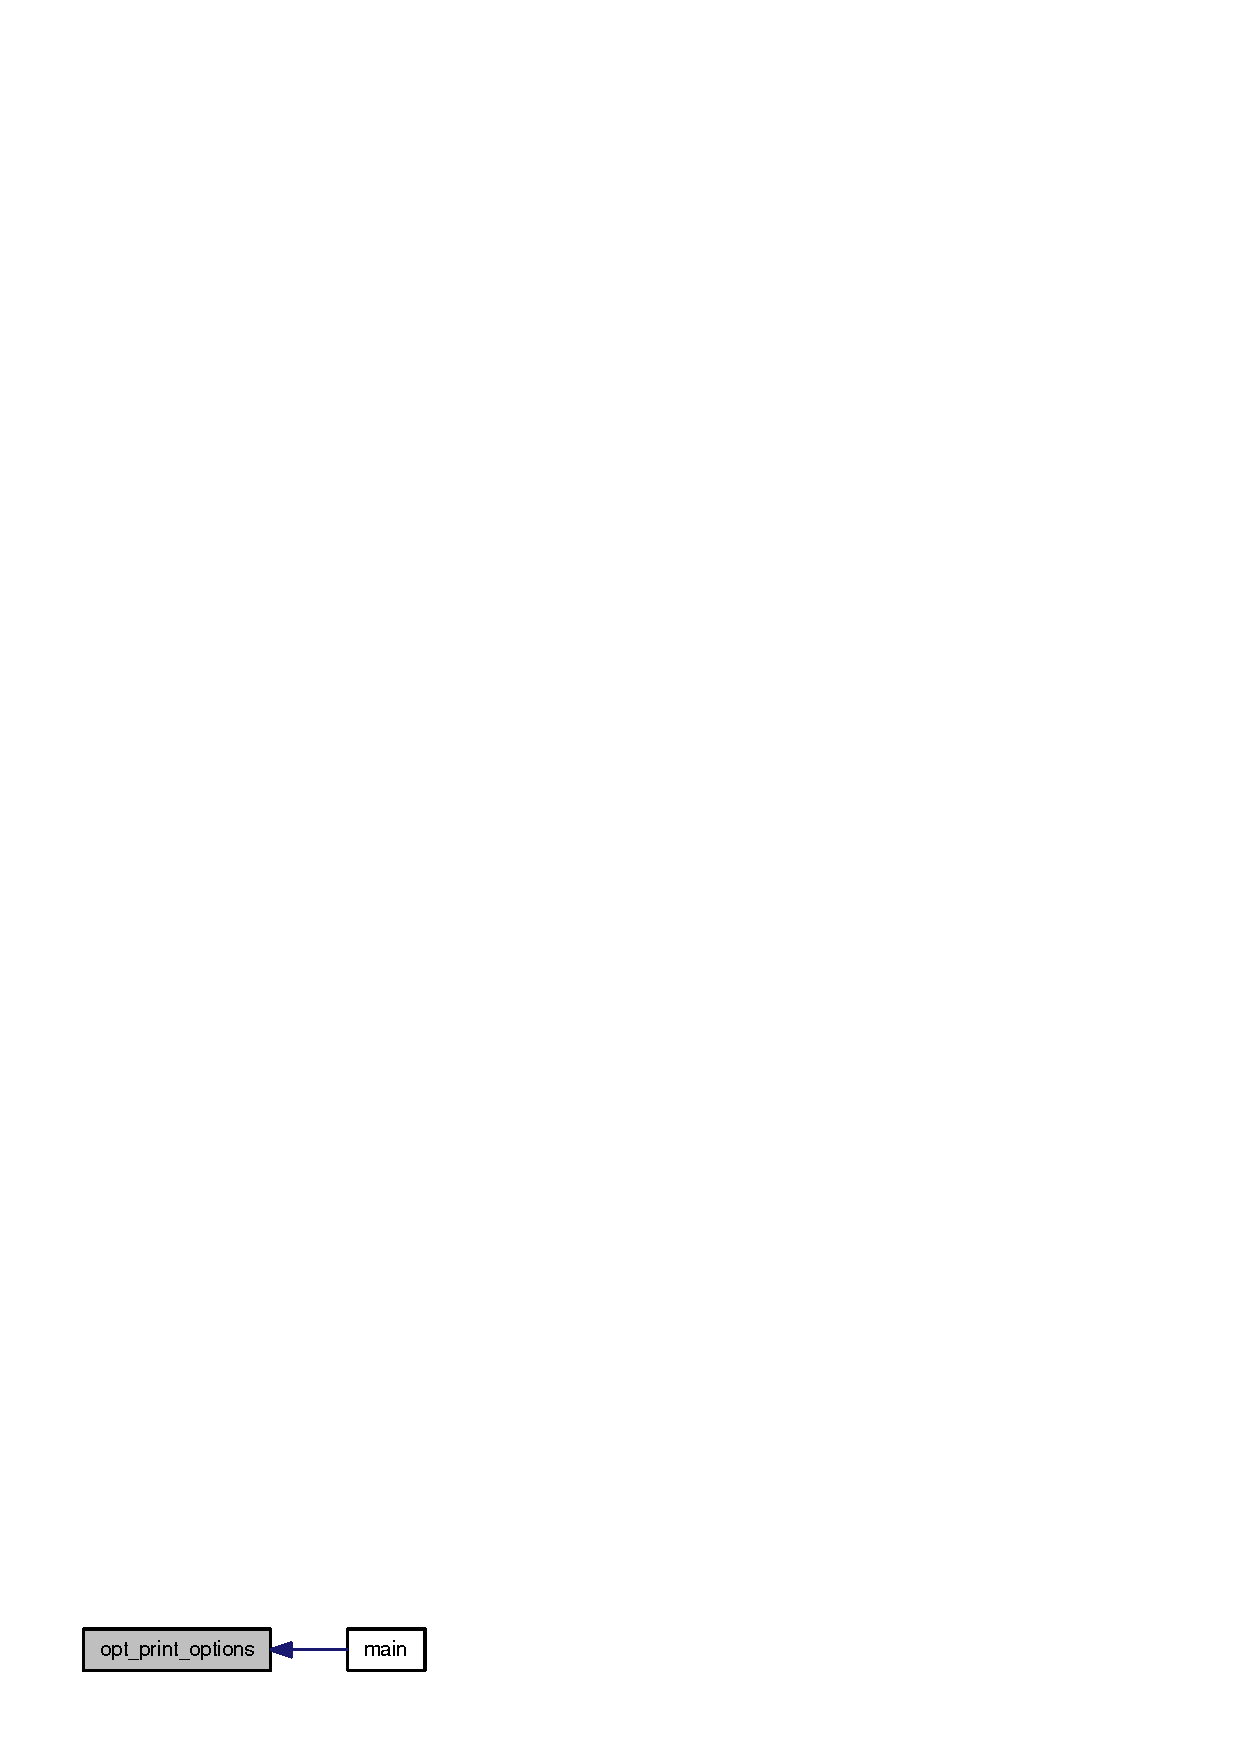
\includegraphics[width=104pt]{options_8h_86b86016ad1396461ed934c0ab462a35_icgraph}
\end{center}
\end{figure}
\index{options.h@{options.h}!opt\_\-process\_\-options@{opt\_\-process\_\-options}}
\index{opt\_\-process\_\-options@{opt\_\-process\_\-options}!options.h@{options.h}}
\subsubsection[{opt\_\-process\_\-options}]{\setlength{\rightskip}{0pt plus 5cm}void opt\_\-process\_\-options (struct {\bf opt\_\-odb\_\-t} $\ast$ {\em odb}, \/  int {\em argc}, \/  char $\ast$$\ast$ {\em argv})}\label{options_8h_d342c32672b6463f360141b0faf981ad}




Referenced by main().

Here is the caller graph for this function:\nopagebreak
\begin{figure}[H]
\begin{center}
\leavevmode
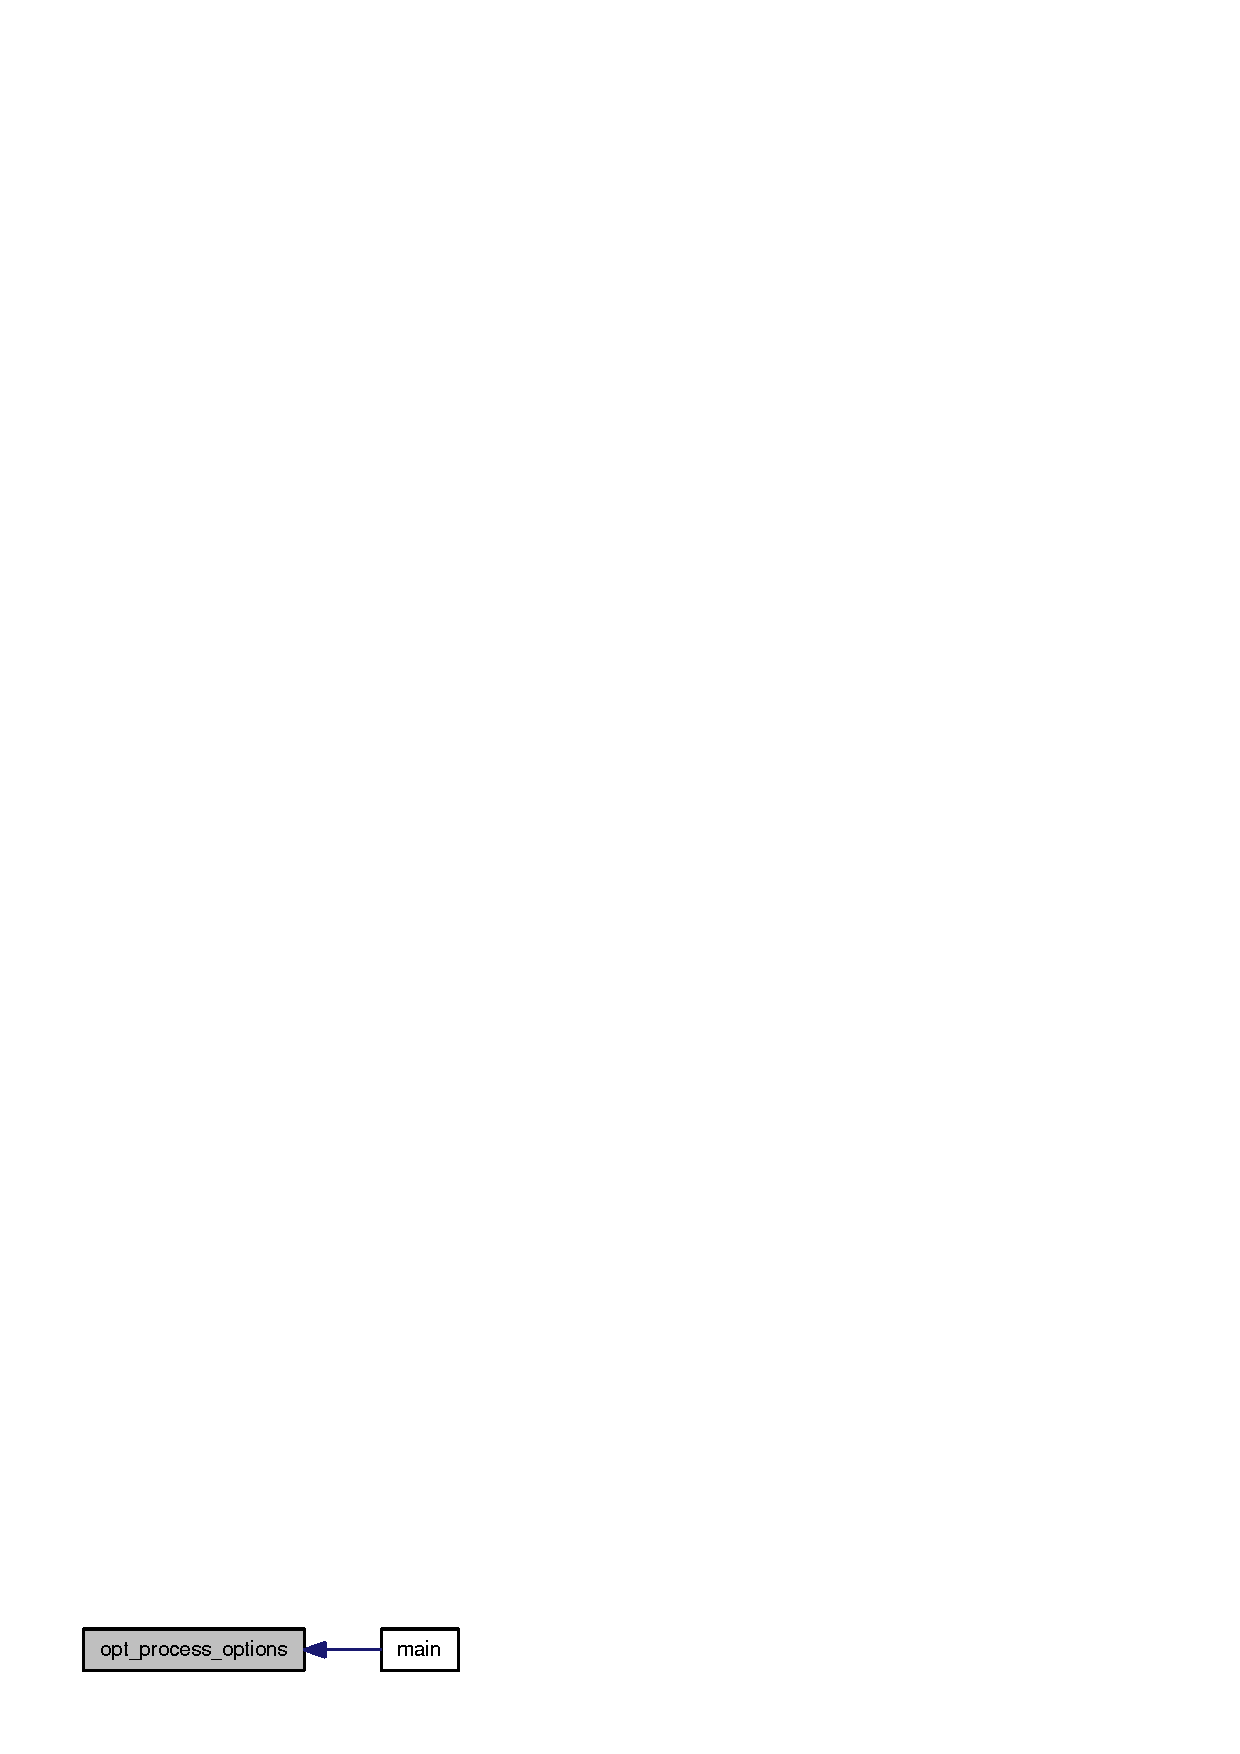
\includegraphics[width=112pt]{options_8h_d342c32672b6463f360141b0faf981ad_icgraph}
\end{center}
\end{figure}
\index{options.h@{options.h}!opt\_\-reg\_\-double@{opt\_\-reg\_\-double}}
\index{opt\_\-reg\_\-double@{opt\_\-reg\_\-double}!options.h@{options.h}}
\subsubsection[{opt\_\-reg\_\-double}]{\setlength{\rightskip}{0pt plus 5cm}void opt\_\-reg\_\-double (struct {\bf opt\_\-odb\_\-t} $\ast$ {\em odb}, \/  char $\ast$ {\em name}, \/  char $\ast$ {\em desc}, \/  double $\ast$ {\em var}, \/  double {\em def\_\-val}, \/  int {\em print}, \/  char $\ast$ {\em format})}\label{options_8h_8b67f54a697dd1f6ad5936220a80b6de}




Referenced by exec\_\-reg\_\-options(), fetch\_\-reg\_\-options(), and uncore\_\-reg\_\-options().

Here is the caller graph for this function:\nopagebreak
\begin{figure}[H]
\begin{center}
\leavevmode
\includegraphics[width=132pt]{options_8h_8b67f54a697dd1f6ad5936220a80b6de_icgraph}
\end{center}
\end{figure}
\index{options.h@{options.h}!opt\_\-reg\_\-double\_\-list@{opt\_\-reg\_\-double\_\-list}}
\index{opt\_\-reg\_\-double\_\-list@{opt\_\-reg\_\-double\_\-list}!options.h@{options.h}}
\subsubsection[{opt\_\-reg\_\-double\_\-list}]{\setlength{\rightskip}{0pt plus 5cm}void opt\_\-reg\_\-double\_\-list (struct {\bf opt\_\-odb\_\-t} $\ast$ {\em odb}, \/  char $\ast$ {\em name}, \/  char $\ast$ {\em desc}, \/  double $\ast$ {\em vars}, \/  int {\em nvars}, \/  int $\ast$ {\em nelt}, \/  double $\ast$ {\em def\_\-val}, \/  int {\em print}, \/  char $\ast$ {\em format}, \/  int {\em accrue})}\label{options_8h_93810182b88f09f4db343557cc4108fe}


\index{options.h@{options.h}!opt\_\-reg\_\-enum@{opt\_\-reg\_\-enum}}
\index{opt\_\-reg\_\-enum@{opt\_\-reg\_\-enum}!options.h@{options.h}}
\subsubsection[{opt\_\-reg\_\-enum}]{\setlength{\rightskip}{0pt plus 5cm}void opt\_\-reg\_\-enum (struct {\bf opt\_\-odb\_\-t} $\ast$ {\em odb}, \/  char $\ast$ {\em name}, \/  char $\ast$ {\em desc}, \/  int $\ast$ {\em var}, \/  char $\ast$ {\em def\_\-val}, \/  char $\ast$$\ast$ {\em emap}, \/  int $\ast$ {\em eval}, \/  int {\em emap\_\-sz}, \/  int {\em print}, \/  char $\ast$ {\em format})}\label{options_8h_0230cf420485a309bef1424117a63410}


\index{options.h@{options.h}!opt\_\-reg\_\-enum\_\-list@{opt\_\-reg\_\-enum\_\-list}}
\index{opt\_\-reg\_\-enum\_\-list@{opt\_\-reg\_\-enum\_\-list}!options.h@{options.h}}
\subsubsection[{opt\_\-reg\_\-enum\_\-list}]{\setlength{\rightskip}{0pt plus 5cm}void opt\_\-reg\_\-enum\_\-list (struct {\bf opt\_\-odb\_\-t} $\ast$ {\em odb}, \/  char $\ast$ {\em name}, \/  char $\ast$ {\em desc}, \/  int $\ast$ {\em vars}, \/  int {\em nvars}, \/  int $\ast$ {\em nelt}, \/  char $\ast$ {\em def\_\-val}, \/  char $\ast$$\ast$ {\em emap}, \/  int $\ast$ {\em eval}, \/  int {\em emap\_\-sz}, \/  int {\em print}, \/  char $\ast$ {\em format}, \/  int {\em accrue})}\label{options_8h_8daa1e40a467b32cf8ccf36880eace16}


\index{options.h@{options.h}!opt\_\-reg\_\-flag@{opt\_\-reg\_\-flag}}
\index{opt\_\-reg\_\-flag@{opt\_\-reg\_\-flag}!options.h@{options.h}}
\subsubsection[{opt\_\-reg\_\-flag}]{\setlength{\rightskip}{0pt plus 5cm}void opt\_\-reg\_\-flag (struct {\bf opt\_\-odb\_\-t} $\ast$ {\em odb}, \/  char $\ast$ {\em name}, \/  char $\ast$ {\em desc}, \/  bool $\ast$ {\em var}, \/  bool {\em def\_\-val}, \/  int {\em print}, \/  char $\ast$ {\em format})}\label{options_8h_67bace6ae10ed0ee002a5efb379ba300}




Referenced by alloc\_\-reg\_\-options(), decode\_\-reg\_\-options(), exec\_\-reg\_\-options(), fetch\_\-reg\_\-options(), and uncore\_\-reg\_\-options().

Here is the caller graph for this function:\nopagebreak
\begin{figure}[H]
\begin{center}
\leavevmode
\includegraphics[width=127pt]{options_8h_67bace6ae10ed0ee002a5efb379ba300_icgraph}
\end{center}
\end{figure}
\index{options.h@{options.h}!opt\_\-reg\_\-flag\_\-list@{opt\_\-reg\_\-flag\_\-list}}
\index{opt\_\-reg\_\-flag\_\-list@{opt\_\-reg\_\-flag\_\-list}!options.h@{options.h}}
\subsubsection[{opt\_\-reg\_\-flag\_\-list}]{\setlength{\rightskip}{0pt plus 5cm}void opt\_\-reg\_\-flag\_\-list (struct {\bf opt\_\-odb\_\-t} $\ast$ {\em odb}, \/  char $\ast$ {\em name}, \/  char $\ast$ {\em desc}, \/  bool $\ast$ {\em vars}, \/  int {\em nvars}, \/  int $\ast$ {\em nelt}, \/  bool $\ast$ {\em def\_\-val}, \/  int {\em print}, \/  char $\ast$ {\em format}, \/  int {\em accrue})}\label{options_8h_51490d3edc932834af7604128f3bd25c}


\index{options.h@{options.h}!opt\_\-reg\_\-float@{opt\_\-reg\_\-float}}
\index{opt\_\-reg\_\-float@{opt\_\-reg\_\-float}!options.h@{options.h}}
\subsubsection[{opt\_\-reg\_\-float}]{\setlength{\rightskip}{0pt plus 5cm}void opt\_\-reg\_\-float (struct {\bf opt\_\-odb\_\-t} $\ast$ {\em odb}, \/  char $\ast$ {\em name}, \/  char $\ast$ {\em desc}, \/  float $\ast$ {\em var}, \/  float {\em def\_\-val}, \/  int {\em print}, \/  char $\ast$ {\em format})}\label{options_8h_c15111fd41a8f520e56180ce7677e6ce}


\index{options.h@{options.h}!opt\_\-reg\_\-float\_\-list@{opt\_\-reg\_\-float\_\-list}}
\index{opt\_\-reg\_\-float\_\-list@{opt\_\-reg\_\-float\_\-list}!options.h@{options.h}}
\subsubsection[{opt\_\-reg\_\-float\_\-list}]{\setlength{\rightskip}{0pt plus 5cm}void opt\_\-reg\_\-float\_\-list (struct {\bf opt\_\-odb\_\-t} $\ast$ {\em odb}, \/  char $\ast$ {\em name}, \/  char $\ast$ {\em desc}, \/  float $\ast$ {\em vars}, \/  int {\em nvars}, \/  int $\ast$ {\em nelt}, \/  float $\ast$ {\em def\_\-val}, \/  int {\em print}, \/  char $\ast$ {\em format}, \/  int {\em accrue})}\label{options_8h_9772b1fbca529f89d3fed92c00159626}


\index{options.h@{options.h}!opt\_\-reg\_\-header@{opt\_\-reg\_\-header}}
\index{opt\_\-reg\_\-header@{opt\_\-reg\_\-header}!options.h@{options.h}}
\subsubsection[{opt\_\-reg\_\-header}]{\setlength{\rightskip}{0pt plus 5cm}void opt\_\-reg\_\-header (struct {\bf opt\_\-odb\_\-t} $\ast$ {\em odb}, \/  char $\ast$ {\em header})}\label{options_8h_e5fc90dec7d9a246d2dded1b0c8ba56d}


\index{options.h@{options.h}!opt\_\-reg\_\-int@{opt\_\-reg\_\-int}}
\index{opt\_\-reg\_\-int@{opt\_\-reg\_\-int}!options.h@{options.h}}
\subsubsection[{opt\_\-reg\_\-int}]{\setlength{\rightskip}{0pt plus 5cm}void opt\_\-reg\_\-int (struct {\bf opt\_\-odb\_\-t} $\ast$ {\em odb}, \/  char $\ast$ {\em name}, \/  char $\ast$ {\em desc}, \/  int $\ast$ {\em var}, \/  int {\em def\_\-val}, \/  int {\em print}, \/  char $\ast$ {\em format})}\label{options_8h_3c40c51f020768250172b4231275584e}




Referenced by alloc\_\-reg\_\-options(), commit\_\-reg\_\-options(), decode\_\-reg\_\-options(), exec\_\-reg\_\-options(), fetch\_\-reg\_\-options(), and uncore\_\-reg\_\-options().

Here is the caller graph for this function:\nopagebreak
\begin{figure}[H]
\begin{center}
\leavevmode
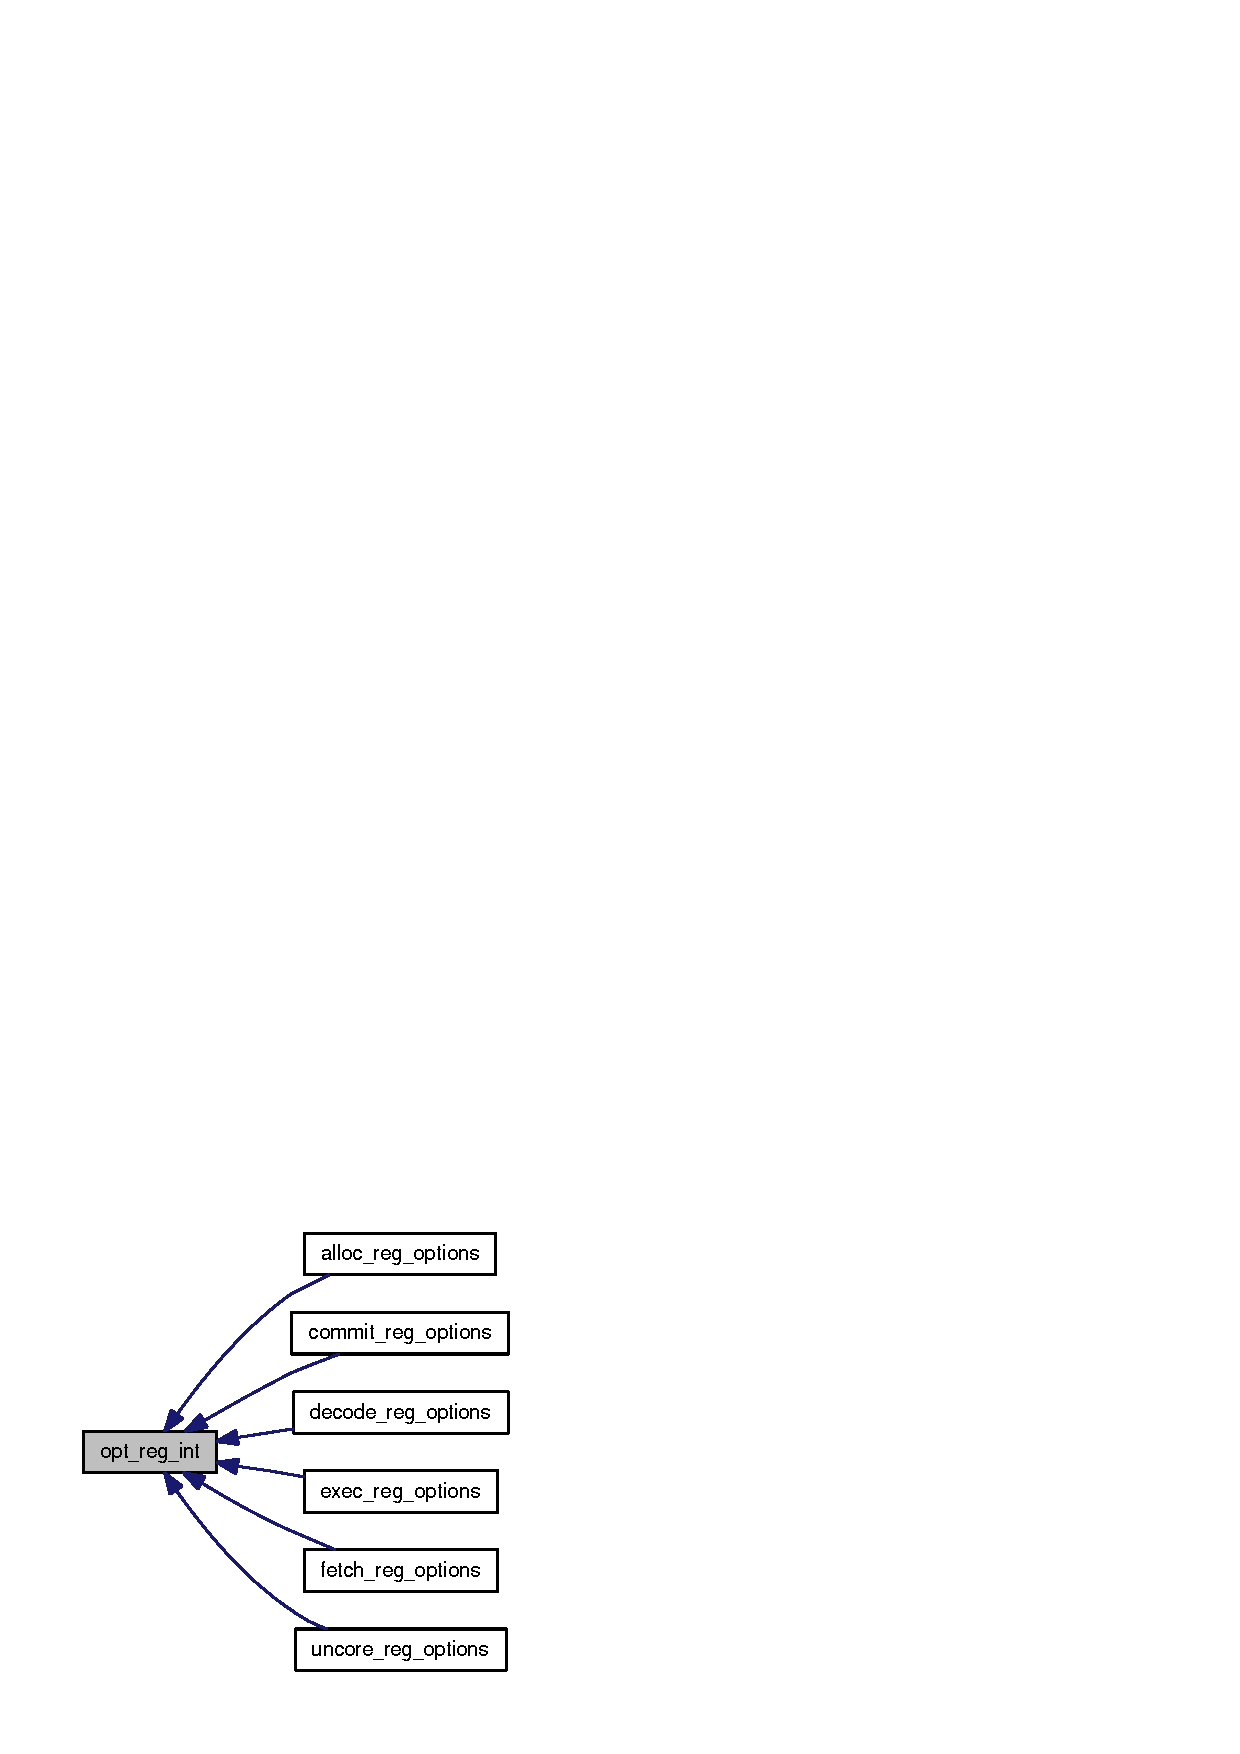
\includegraphics[width=124pt]{options_8h_3c40c51f020768250172b4231275584e_icgraph}
\end{center}
\end{figure}
\index{options.h@{options.h}!opt\_\-reg\_\-int\_\-list@{opt\_\-reg\_\-int\_\-list}}
\index{opt\_\-reg\_\-int\_\-list@{opt\_\-reg\_\-int\_\-list}!options.h@{options.h}}
\subsubsection[{opt\_\-reg\_\-int\_\-list}]{\setlength{\rightskip}{0pt plus 5cm}void opt\_\-reg\_\-int\_\-list (struct {\bf opt\_\-odb\_\-t} $\ast$ {\em odb}, \/  char $\ast$ {\em name}, \/  char $\ast$ {\em desc}, \/  int $\ast$ {\em vars}, \/  int {\em nvars}, \/  int $\ast$ {\em nelt}, \/  int $\ast$ {\em def\_\-val}, \/  int {\em print}, \/  char $\ast$ {\em format}, \/  int {\em accrue})}\label{options_8h_60f1bb4c4b37899e70b8250dfd5c7df7}




Referenced by decode\_\-reg\_\-options(), and exec\_\-reg\_\-options().

Here is the caller graph for this function:\nopagebreak
\begin{figure}[H]
\begin{center}
\leavevmode
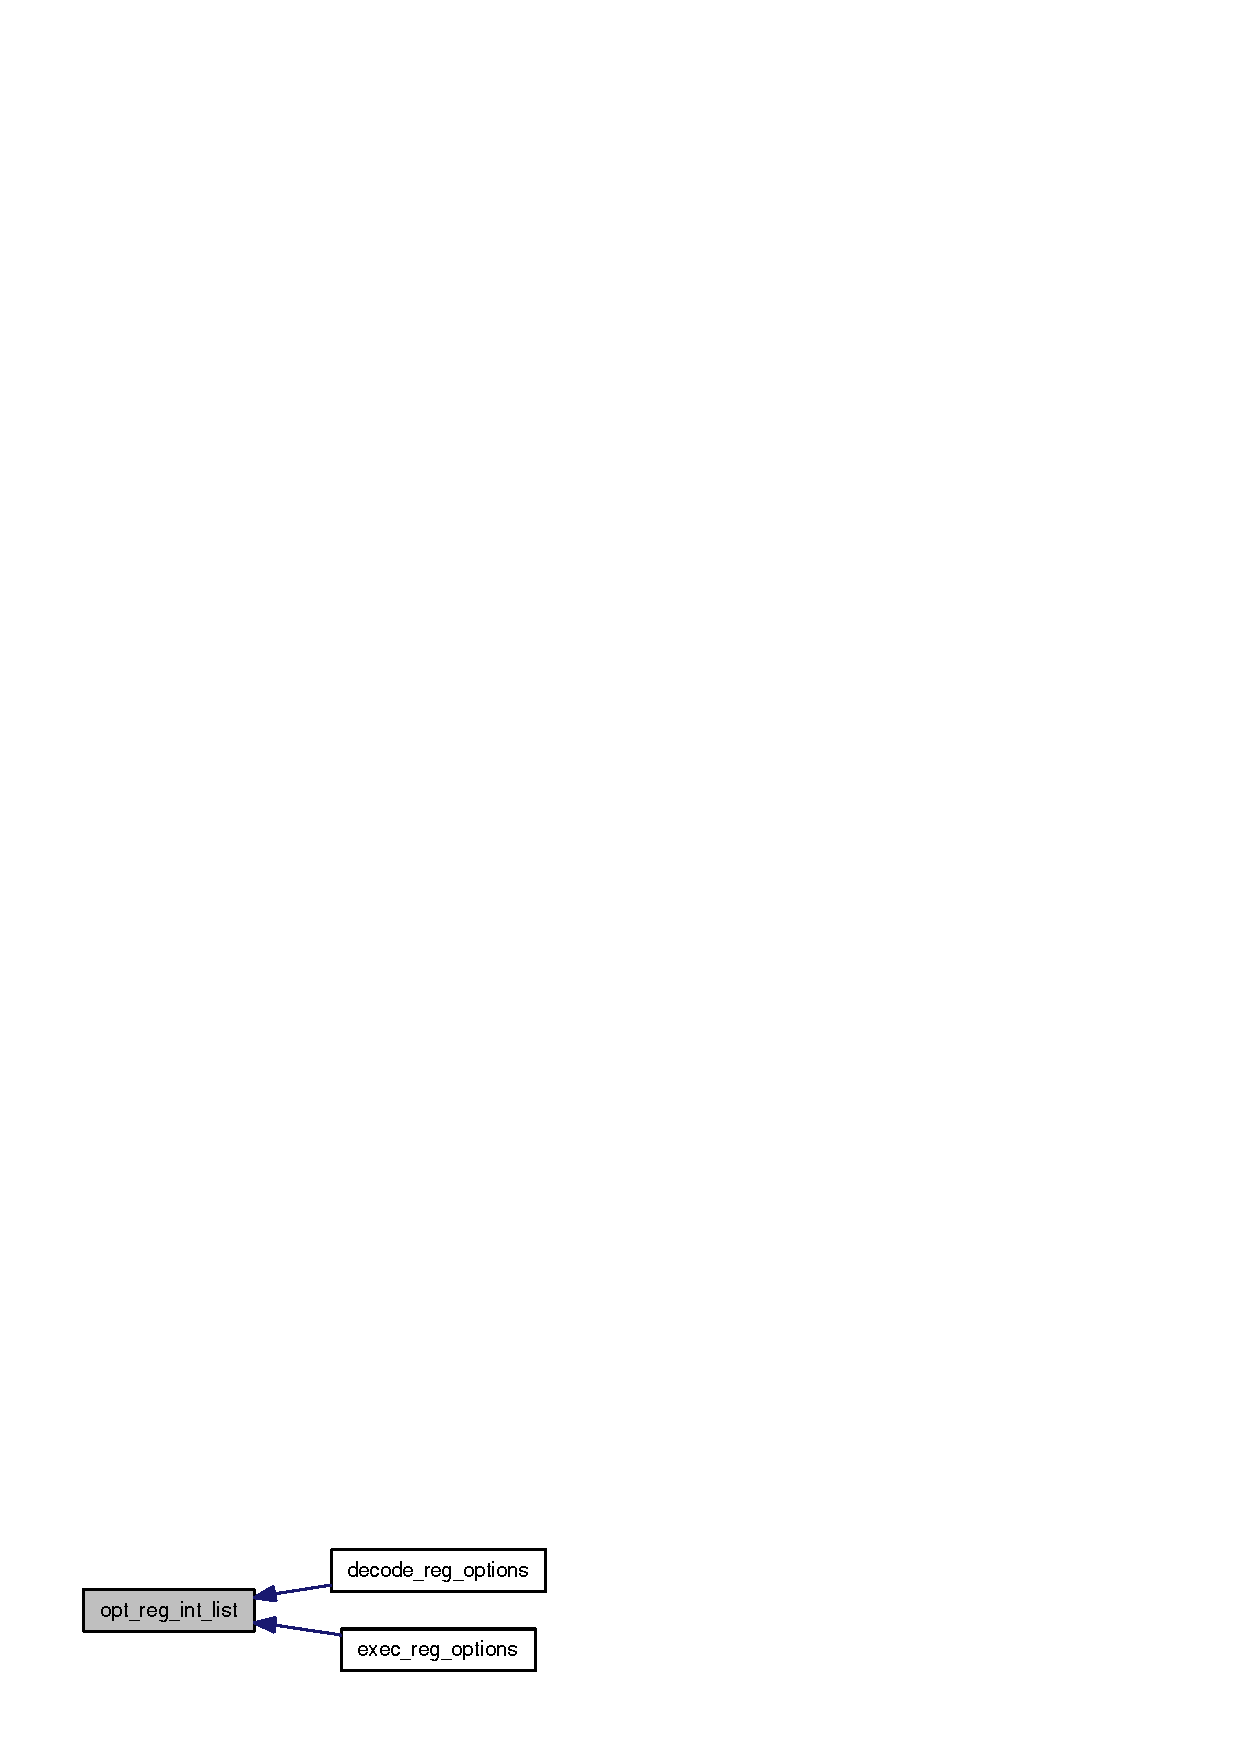
\includegraphics[width=133pt]{options_8h_60f1bb4c4b37899e70b8250dfd5c7df7_icgraph}
\end{center}
\end{figure}
\index{options.h@{options.h}!opt\_\-reg\_\-long\_\-long@{opt\_\-reg\_\-long\_\-long}}
\index{opt\_\-reg\_\-long\_\-long@{opt\_\-reg\_\-long\_\-long}!options.h@{options.h}}
\subsubsection[{opt\_\-reg\_\-long\_\-long}]{\setlength{\rightskip}{0pt plus 5cm}void opt\_\-reg\_\-long\_\-long (struct {\bf opt\_\-odb\_\-t} $\ast$ {\em odb}, \/  char $\ast$ {\em name}, \/  char $\ast$ {\em desc}, \/  long long $\ast$ {\em var}, \/  long long {\em def\_\-val}, \/  int {\em print}, \/  char $\ast$ {\em format})}\label{options_8h_1272c126bc4795af0d6dcdca2e980356}


\index{options.h@{options.h}!opt\_\-reg\_\-note@{opt\_\-reg\_\-note}}
\index{opt\_\-reg\_\-note@{opt\_\-reg\_\-note}!options.h@{options.h}}
\subsubsection[{opt\_\-reg\_\-note}]{\setlength{\rightskip}{0pt plus 5cm}void opt\_\-reg\_\-note (struct {\bf opt\_\-odb\_\-t} $\ast$ {\em odb}, \/  char $\ast$ {\em note})}\label{options_8h_82f126f3dc50479ca8e9ed237da85e7a}


\index{options.h@{options.h}!opt\_\-reg\_\-string@{opt\_\-reg\_\-string}}
\index{opt\_\-reg\_\-string@{opt\_\-reg\_\-string}!options.h@{options.h}}
\subsubsection[{opt\_\-reg\_\-string}]{\setlength{\rightskip}{0pt plus 5cm}void opt\_\-reg\_\-string (struct {\bf opt\_\-odb\_\-t} $\ast$ {\em odb}, \/  char $\ast$ {\em name}, \/  char $\ast$ {\em desc}, \/  char $\ast$$\ast$ {\em var}, \/  char $\ast$ {\em def\_\-val}, \/  int {\em print}, \/  char $\ast$ {\em format})}\label{options_8h_a2015efb5a683bc3f45b63dd94a58b97}




Referenced by dram\_\-reg\_\-options(), exec\_\-reg\_\-options(), fetch\_\-reg\_\-options(), and uncore\_\-reg\_\-options().

Here is the caller graph for this function:\nopagebreak
\begin{figure}[H]
\begin{center}
\leavevmode
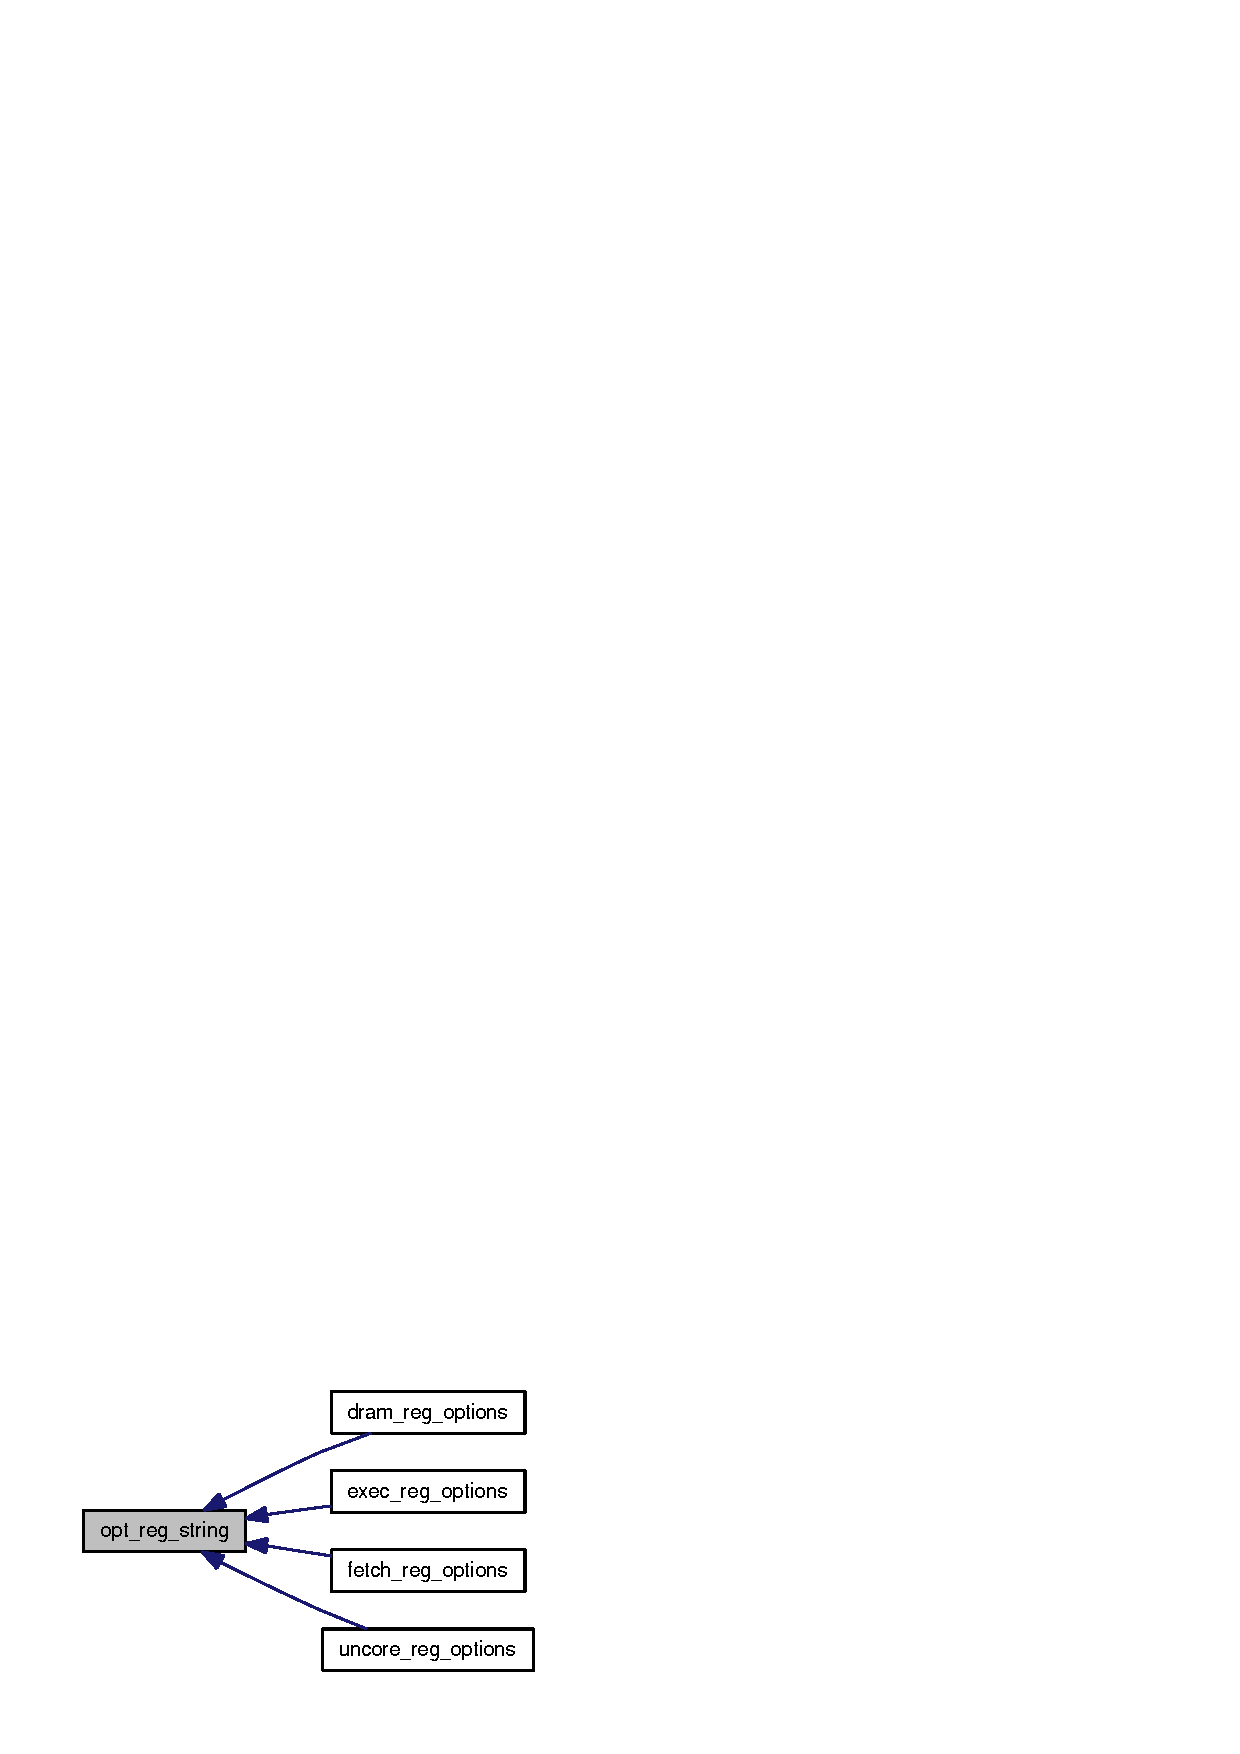
\includegraphics[width=130pt]{options_8h_a2015efb5a683bc3f45b63dd94a58b97_icgraph}
\end{center}
\end{figure}
\index{options.h@{options.h}!opt\_\-reg\_\-string\_\-list@{opt\_\-reg\_\-string\_\-list}}
\index{opt\_\-reg\_\-string\_\-list@{opt\_\-reg\_\-string\_\-list}!options.h@{options.h}}
\subsubsection[{opt\_\-reg\_\-string\_\-list}]{\setlength{\rightskip}{0pt plus 5cm}void opt\_\-reg\_\-string\_\-list (struct {\bf opt\_\-odb\_\-t} $\ast$ {\em odb}, \/  char $\ast$ {\em name}, \/  char $\ast$ {\em desc}, \/  char $\ast$$\ast$ {\em vars}, \/  int {\em nvars}, \/  int $\ast$ {\em nelt}, \/  char $\ast$$\ast$ {\em def\_\-val}, \/  int {\em print}, \/  char $\ast$ {\em format}, \/  int {\em accrue})}\label{options_8h_752ea4c2b38f9ed0bb1126b7b23ac869}




Referenced by exec\_\-reg\_\-options(), fetch\_\-reg\_\-options(), and uncore\_\-reg\_\-options().

Here is the caller graph for this function:\nopagebreak
\begin{figure}[H]
\begin{center}
\leavevmode
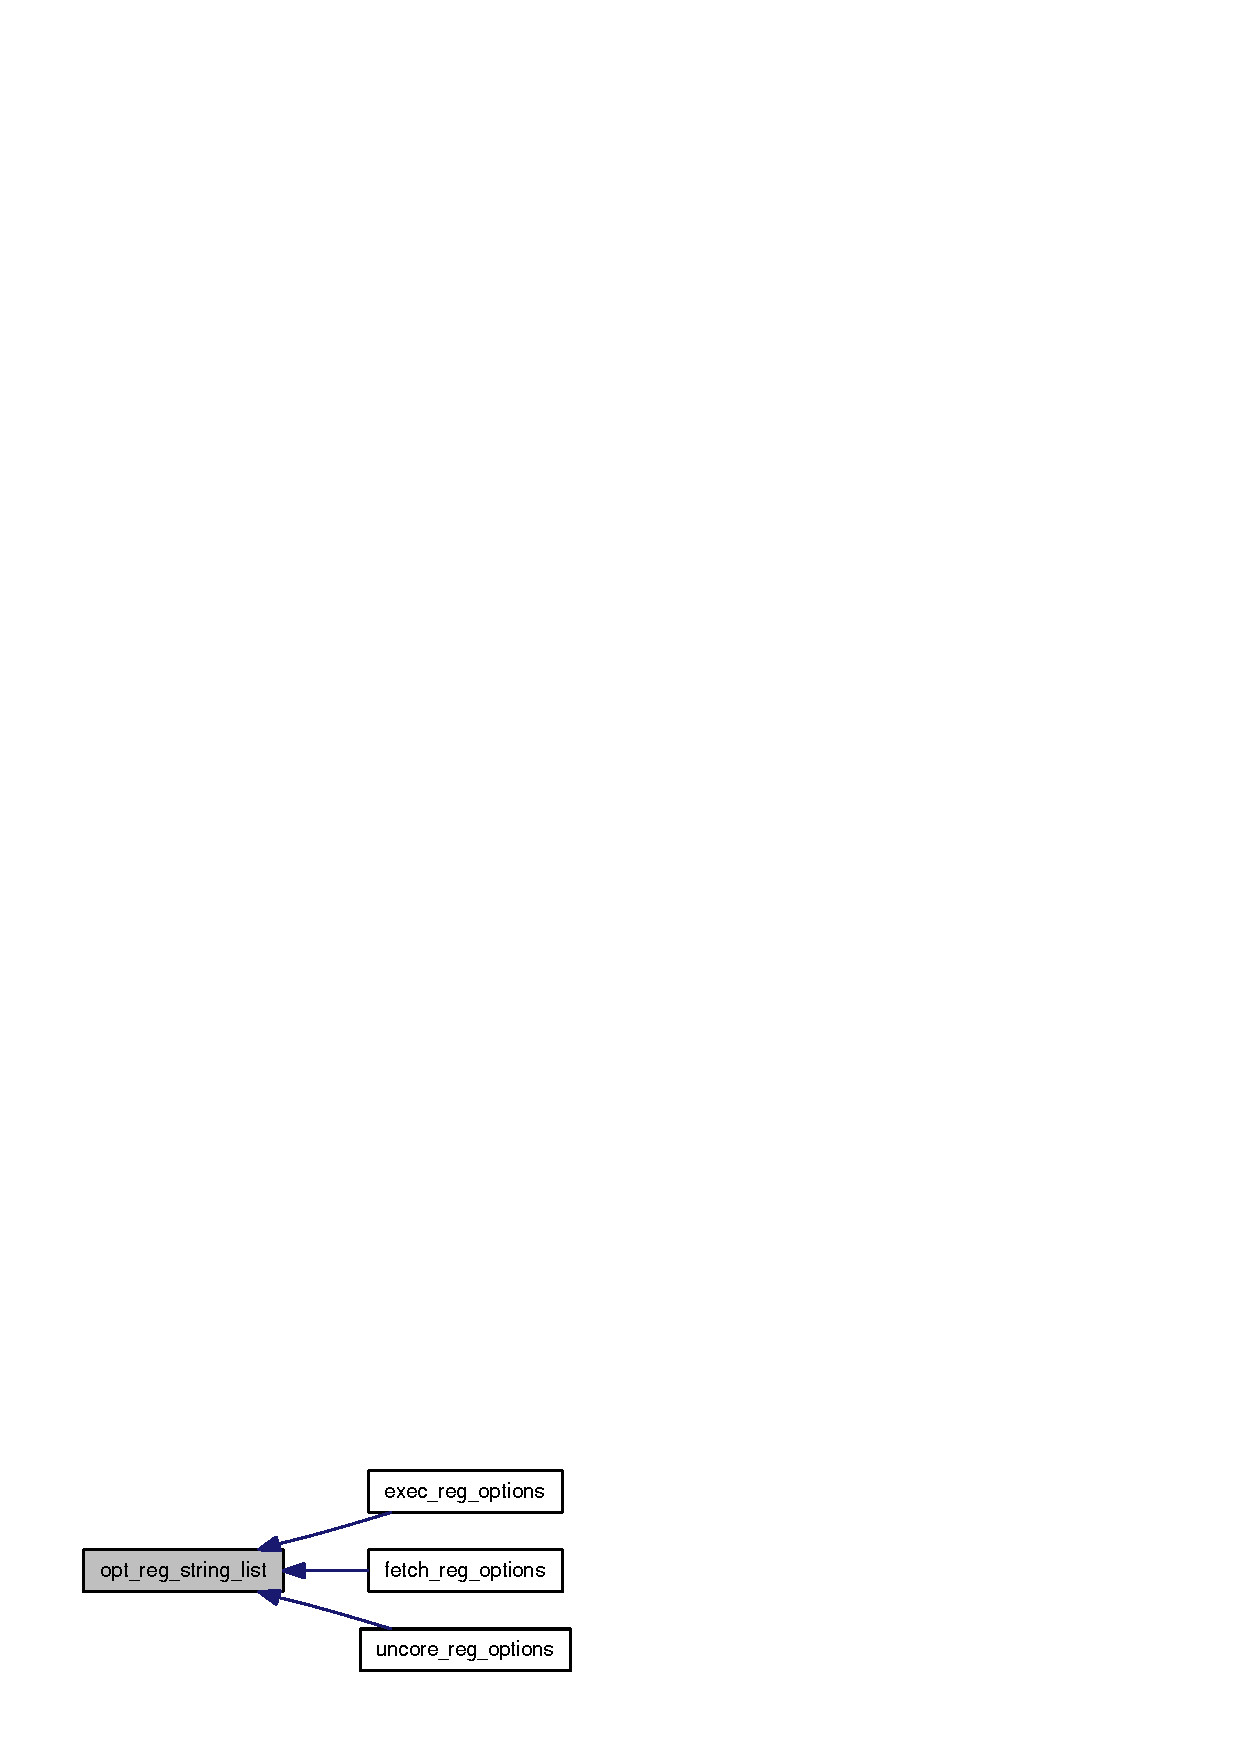
\includegraphics[width=139pt]{options_8h_752ea4c2b38f9ed0bb1126b7b23ac869_icgraph}
\end{center}
\end{figure}
\index{options.h@{options.h}!opt\_\-reg\_\-uint@{opt\_\-reg\_\-uint}}
\index{opt\_\-reg\_\-uint@{opt\_\-reg\_\-uint}!options.h@{options.h}}
\subsubsection[{opt\_\-reg\_\-uint}]{\setlength{\rightskip}{0pt plus 5cm}void opt\_\-reg\_\-uint (struct {\bf opt\_\-odb\_\-t} $\ast$ {\em odb}, \/  char $\ast$ {\em name}, \/  char $\ast$ {\em desc}, \/  unsigned int $\ast$ {\em var}, \/  unsigned int {\em def\_\-val}, \/  int {\em print}, \/  char $\ast$ {\em format})}\label{options_8h_9507998320eb91ad361735d2120eb4fd}


\index{options.h@{options.h}!opt\_\-reg\_\-uint\_\-list@{opt\_\-reg\_\-uint\_\-list}}
\index{opt\_\-reg\_\-uint\_\-list@{opt\_\-reg\_\-uint\_\-list}!options.h@{options.h}}
\subsubsection[{opt\_\-reg\_\-uint\_\-list}]{\setlength{\rightskip}{0pt plus 5cm}void opt\_\-reg\_\-uint\_\-list (struct {\bf opt\_\-odb\_\-t} $\ast$ {\em odb}, \/  char $\ast$ {\em name}, \/  char $\ast$ {\em desc}, \/  unsigned int $\ast$ {\em vars}, \/  int {\em nvars}, \/  int $\ast$ {\em nelt}, \/  unsigned int $\ast$ {\em def\_\-val}, \/  int {\em print}, \/  char $\ast$ {\em format}, \/  int {\em accrue})}\label{options_8h_8ba54cb3d259cbe1c0faa57a55d510c7}




\subsection{Variable Documentation}
\index{options.h@{options.h}!opt\_\-ignore\_\-notes@{opt\_\-ignore\_\-notes}}
\index{opt\_\-ignore\_\-notes@{opt\_\-ignore\_\-notes}!options.h@{options.h}}
\subsubsection[{opt\_\-ignore\_\-notes}]{\setlength{\rightskip}{0pt plus 5cm}bool {\bf opt\_\-ignore\_\-notes}}\label{options_8h_c2771665f9c910976267026901cb2355}


